\section{Bestandsmanagement}

\subsection{Produktionsprogrammplanung}
\textbf{Definition:} Produktionsprogrammplanung legt fest in welchen Arten, Mengen
und in welcher zeitlichen Verteilung hergestellt wird.

\textbf{Zeitliche Ebenen der Produktionsprogrammplanung:}
\begin{itemize}
	\item \textbf{Strategisch}: Festlegung der Produktfelder
	\item \textbf{Taktisch}: Konkretisierung der Produktfelder, Festlegung der Breite und Tiefe
	\item \textbf{Operativ}: Festlegung der Art und Menge der zu produzierenden Erzeugnisse
	für die nächste Planungsperiode $\rightarrow$ \textbf{Frage}: Welches Produktionsprogramm maximiert bei gegebenen Kapazitäten und Deckungsbeiträgen pro Produkt den Gesamtdeckungsbeitrag?
\end{itemize}
\bigskip
\textbf{Deckungsbeitrag:}
\begin{itemize}
	\item (Gesamt-) Gewinn $=$ Erlös $–$ Kosten $=$ Erlös $–$ (Fixkosten $+$ variable Kosten)
	\item Stückgewinn $=$ Stückerlös $–$ Stückkosten $=$ Stückerlös $–$ (Fixkosten pro Stück $+$ variable Stückkosten)
	\item \textbf{Deckungsbeitrag} $=$ Stückerlös $–$ variable Stückkosten
	\item Wenn die Summe aller erzielten Deckungsbeiträge die gesamten Fixkosten abdeckt, wird die \textbf{Gewinnschwelle} erreicht
\end{itemize}
\bigskip
\textbf{Berechnung des optimalen Produktionsprogramm:} \textit{siehe Produktion VL 2, F9-15} \textbf{WICHTIG}! $\rightarrow$ Lösung mit Simplex-Algorithmus (\textit{s. Logistik Tut} 1) oder Eckpunktmethode oder grafisch

\subsection{Bedarfsermittlung}

\textbf{Ziel:} Zeitgerechte, exakte Ermittlung der benötigten Güter (und Dienstleistungen), um die Versorgungssicherheit entlang von Wertschöpfungsketten zu gewährleisten

\textbf{Verfahren der Materialbedarfsermittlung:}
\begin{itemize}
	\item \textbf{Produktionsprogrammgesteuerte Bedarfsermittlung}: Programmgebunden, Basierend auf dem aktuellen Produktionsprogramm, Deterministisch
	\item \textbf{Verbrauchsorientierte Bedarfsermittlung}: Verbrauchsgebunden, Basierend auf dem Bedarf in der Vergangenheit oder Prognosen der Zukunft, Stochastisch möglich
\end{itemize}
\bigskip
\textbf{Produktionsprogrammgesteuerte Bedarfsermittlung:}
\begin{center}
	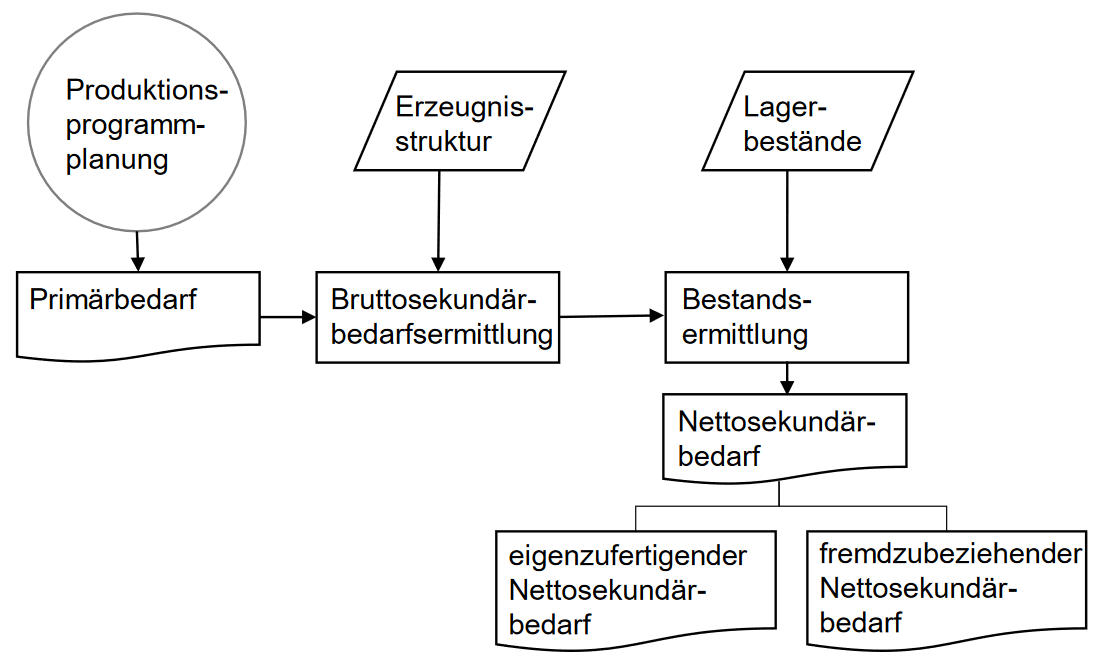
\includegraphics[width=0.6\textwidth]{images/pp-bedarfsermittlung.png}
\end{center}
\textbf{Beispiel}: Primärbedarf = 5 Fahrräder, Erzeugnisstruktur = Zusammensetzung eines Fahrrads, Bruttosekundärbedarf = z.B. Anzahl Räder, Nettosekundärbedarf = Bruttosekundärbedarf abzüglich den Bauteilen, die im Lager vorhanden sind

\textit{Konkrete Berechnung s. Produktion Tut 1}\\

\textbf{Stücklistenauflösung und Gozinto-Graph:}
\begin{itemize}
	\item Beschreibung der Mengenrelationen zwischen Endprodukten, Baugruppen und Einzelteilen
	\item Unterscheide \textbf{mehrteilige Fertigung} (Endprodukt aus unterschiedlichen Teilen) und \textbf{mehrstufige Fertigung} (Fertigung über mehrere Stufen)
\end{itemize}
\begin{center}
	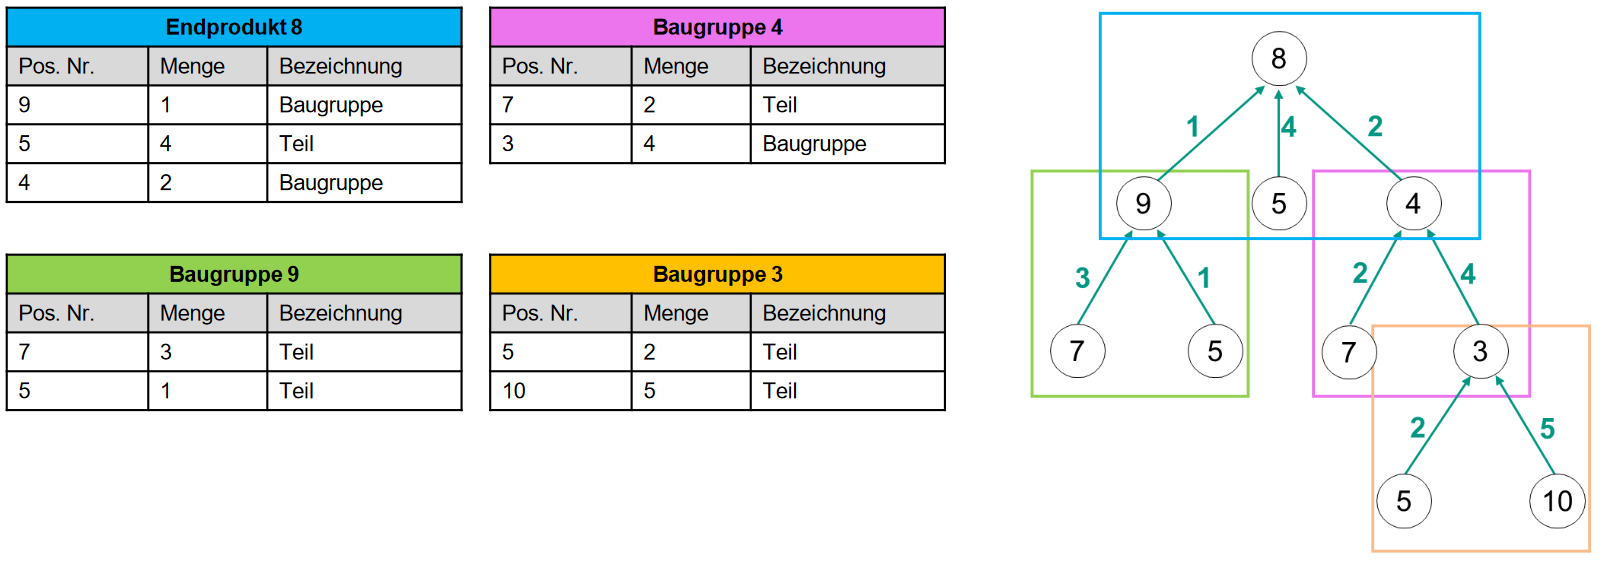
\includegraphics[width=0.8\textwidth]{images/gozinto.png}
\end{center}

\textbf{Verbrauchsorientierte Bedarfsermittlung:}
Angewendet, wenn
\begin{itemize}
	\item Stücklisten nicht vollständig vorhanden sind
	\item der geringe Materialwert eine programmorientierte Ermittlung nicht rechtfertigt
\end{itemize}

Prognosen zeichnen sich durch zwei \textbf{Fehlerrisiken} aus: 
\begin{itemize}
	\item Vorhersagbarkeit zukünftiger Bedarfe
	\item Adäquate mathematische Modellierung
\end{itemize}
\bigskip
\textbf{Methoden der verbrauchsorientierten Bedarfsermittlung:}

Gute Anwendbarkeit:
\begin{itemize}
	\item Arithmetisches Mittel
	\item Gleitender Durschnitt
	\item Exponentielle Glättung (1. Ordnung)
\end{itemize}
Komplexe Methoden:
\begin{itemize}
	\item Exponentielle Glättung (2. Ordnung)
	\item Zeitreihenmodelle wie z. B. ARIMA
\end{itemize}
\textit{Konkrete Berechnung s. Produktion Tut 1}

\subsection{Beschaffungsplanung}
\textbf{Funktion:} Versorgung der Produktion mit den notwendigen Produktionsfaktoren, insb. dem notwendigen Material

\textbf{Teilaufgaben:}
\begin{itemize}
	\item \textbf{Materialbedarfsermittlung}: Ableitung der notwendigen Materialmengen aus dem Produktionsprogramm
	\item \textbf{Losgrößenplanung}: Bündelung der mit der Materialbedarfsermittlung berechneten Bedarfe bei Eigenerstellung von Vorprodukten zu Produktionslosen (Serien)
	\item \textbf{Lagerhaltung}: Puffer zwischen Beschaffung und Produktion
	\item \textbf{Materialwirtschaft}: Organisation der Materialbeschaffung
\end{itemize}
\bigskip
\textbf{Kosten der Beschaffung:}
\begin{itemize}
	\item \textbf{Pagatorische Kosten}: Kosten können nur vorliegen, wenn mit ihnen Auszahlungen verbunden sind
	\item Pagatorische Kosten der Beschaffung:
	\begin{itemize}
		\item Variable Kosten der beschafften Güter und Dienstleistungen
		\item Fixkosten des Lagers
		\item Bestellfixe Kosten (unabhängig von der Bestellmenge)
		\item Variable Lagerhaltungskosten (Kosten durch Verderb und Schwund)
	\end{itemize}
\end{itemize}
\bigskip
\textbf{Beschaffungsarten:}
\begin{itemize}
	\item \textbf{Fallweise Beschaffung}:
	\begin{itemize}
		\item Material wird bei Bedarf beim Lieferanten bestellt
		\item \textbf{Vorteil}: Vermeidung von Lagerhaltungskosten
		\item \textbf{Nachteil}: Mögliche Produktionsausfälle bei Lieferschwierigkeiten und hoher Bestellaufwand
	\end{itemize}
	\item \textbf{Vorratsbeschaffung (Lagerhaltung)}:
	\begin{itemize}
		\item Material wir auf Vorrat bestellt und der Fertigung direkt aus dem Lager zur Verfügung gestellt
		\item \textbf{Vorteil}: Höhere Versorgungssicherheit
		\item \textbf{Nachteil}: Höhere Lagerhaltungskosten
	\end{itemize}
	\item \textbf{Fertigungssynchrone Beschaffung (Just-in-Time)}:
	\begin{itemize}
		\item Rahmenvertrag über längerfristige Abnahmemenge; Material wird jeweils so zeitnah angeliefert, dass es direkt in der Fertigung eingesetzt werden kann
		\item \textbf{Vorteil}: Hohe Versorgungssicherheit bei geringen Lagerkosten
		\item \textbf{Nachteil}: Hoher Planungs-, Abstimmungs- und Transportaufwand
	\end{itemize}
\end{itemize}
\bigskip
\textbf{ABC-Analyse zur Materialklassifikation:}
\begin{itemize}
	\item \textbf{Beobachtung}: Relativ kleiner Teil der zu beschaffenden Güterarten macht den Hauptanteil am gesamten Beschaffungswert aus
	\item Einteilung in A-Güter, B-Güter und C-Güter
	\begin{center}
		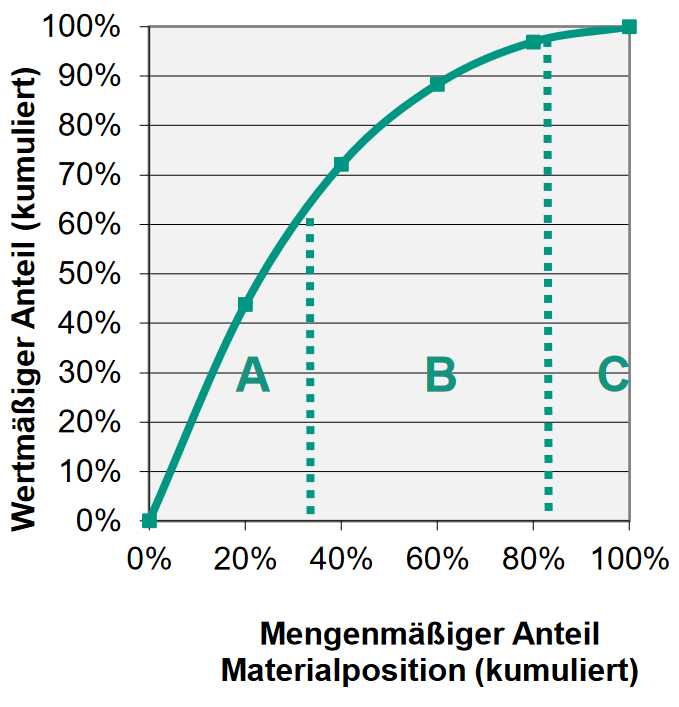
\includegraphics[width=0.4\textwidth]{images/abc.png}
	\end{center}
	\item A-Güter: 
	\begin{itemize}
		\item Fertigungssynchrone Beschaffung, wenn Bedarf stetig und Produktion gut planbar
		\item Fallweise Beschaffung, wenn Bedarf stark schwankend oder Produktionstypen auftragsbezogen sind
		\item Programmgebundene Disposition
	\end{itemize}
	\item C-Güter sollten auf Vorrat beschafft und eingelagert werden, verbrauchsorientierte Beschaffung
	\item Beschaffungsart für B-Güter individuell wählen
\end{itemize}
\bigskip
\textbf{Losgrößenplanung:}
\begin{itemize}
	\item \textbf{Definition Losgröße}: Menge identischer Produktkomponenten, die zwischen zwei Umrüstvorgängen auf einer Produktionsanlage ohne Unterbrechung hergestellt wird
	\item Beispiel: Stelle ich 20 Räder in einem Block oder in 2 Losen je 10 Räder her?
	\item \textbf{Aufgabe}: Ermittlung optimaler Losgrößen, sodass Kosten minimiert werden
	\begin{center}
		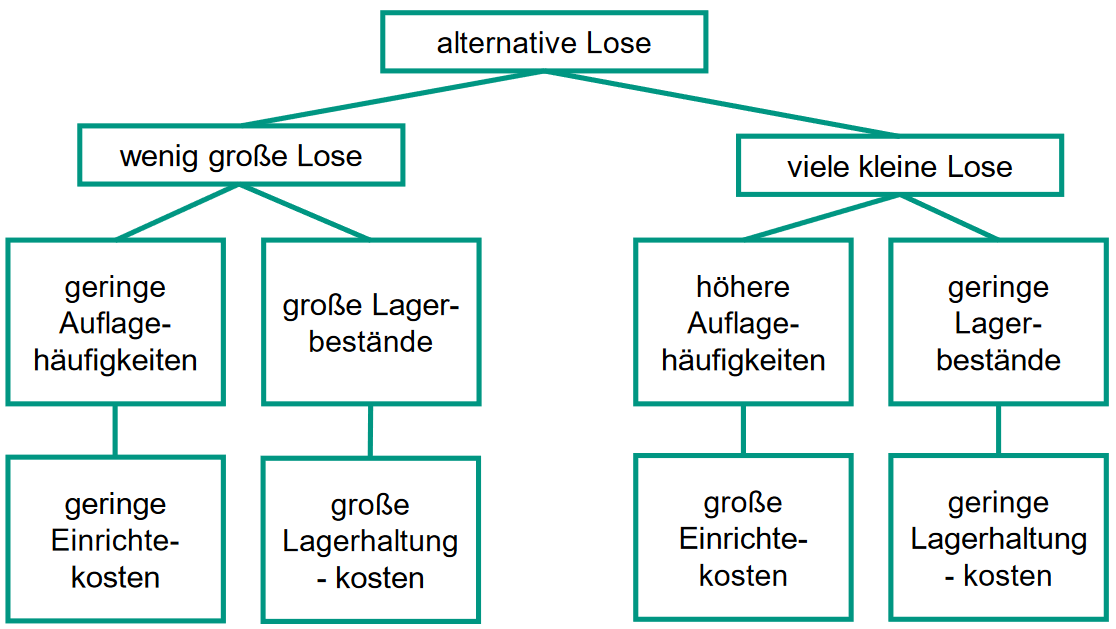
\includegraphics[width=0.6\textwidth]{images/losgröße.png}
	\end{center}
\end{itemize}

\textbf{Einteilung der bei Fremdbeschaffung / Eigenfertigung anfallenden Kosten:}
\begin{itemize}
	\item Beschaffungskosten / variable Produktionskosten:
	\begin{center}
		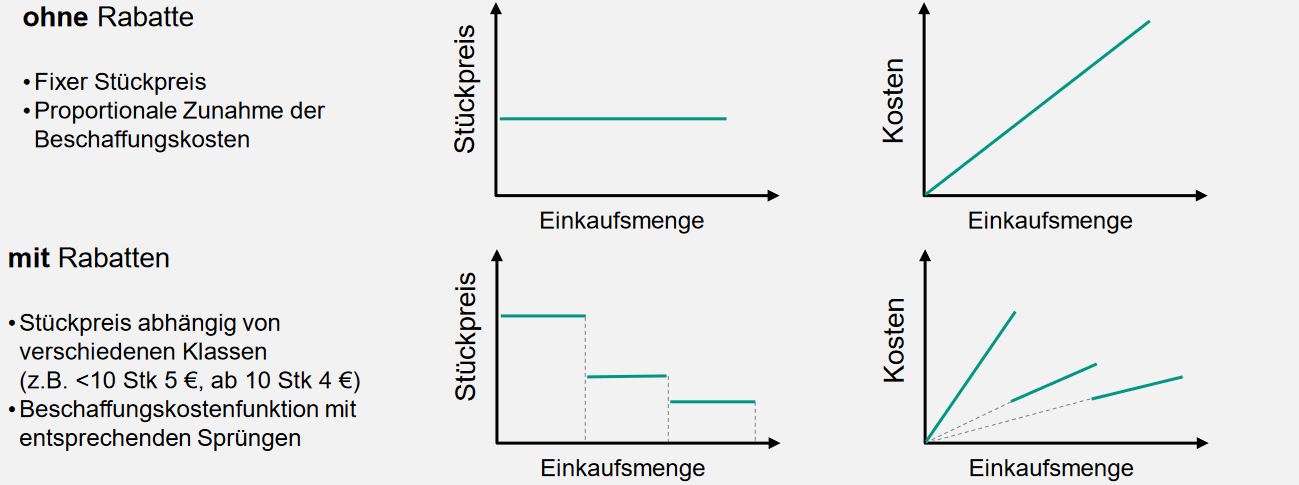
\includegraphics[width=0.7\textwidth]{images/beschaffungskosten.png}
	\end{center}
	\item Bestellkosten / Umrüstkosten: Sind Fixkosten
	\item Lagerhaltungskosten: Beinhaltet neben eigentlichen Lagerkosten auch \textbf{kalkulatorische Zinsen} (Kosten des im Lagerbestand gebundenen Kapitals)
	\item Fehlmengenkosten: Fallen an, wenn das beschaffte Material nicht ausreicht, um den Bedarf der Fertigung zu decken, z.B. entgangene Gewinne
\end{itemize}

\textbf{Lagerhaltung:}
\begin{center}
	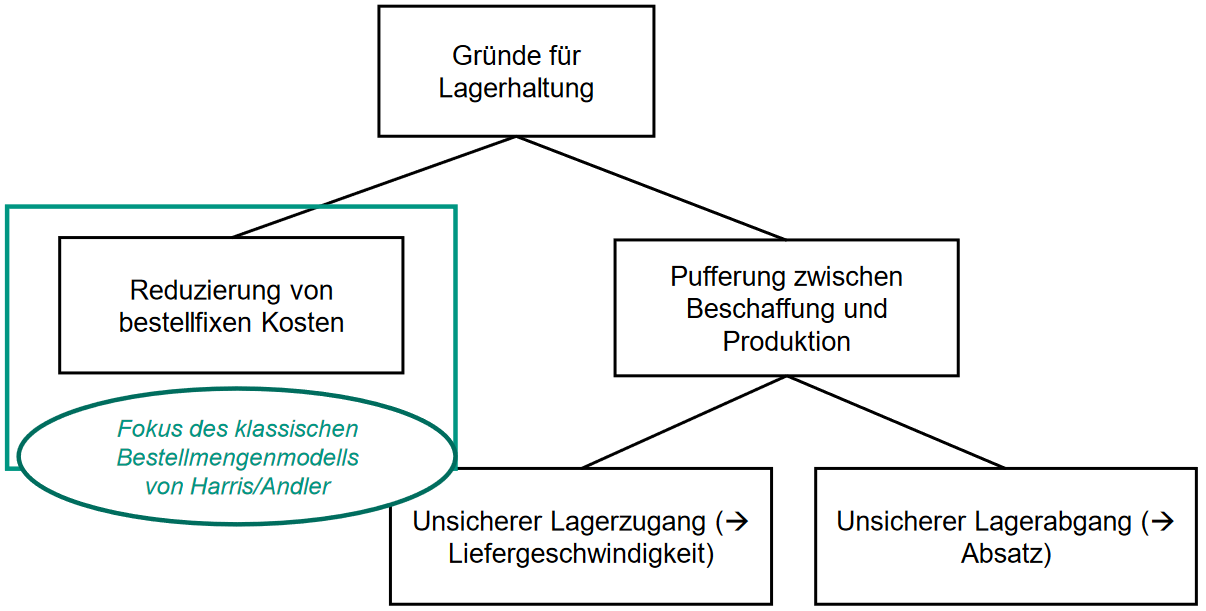
\includegraphics[width=0.7\textwidth]{images/lagerhaltung.png}
\end{center}

\textbf{Harris/Andler-Bestellmengenmodell:}

\textbf{Annahmen}:
\begin{itemize}
	\item Nur ein Gut betrachtet
	\item Beschaffungspreis des Gutes ist unabhängig von der Bestellmenge 
	\item Periodenbedarf ist bekannt
	\item Keine Lieferfristen
	\item Lageranfangsbestand ist gleich Null
	\item Keine Fehlmengen
	\item Keine Kapazitätsbeschränkungen
	\item Keine Unteilbarkeiten hinsichtlich Bestellmenge
	\item Materialverbrauch ist in der Periode konstant / Lagerabgang erfolgt gleichmäßig 
\end{itemize}

\textbf{Lagerbestandsentwicklung:}
\begin{center}
	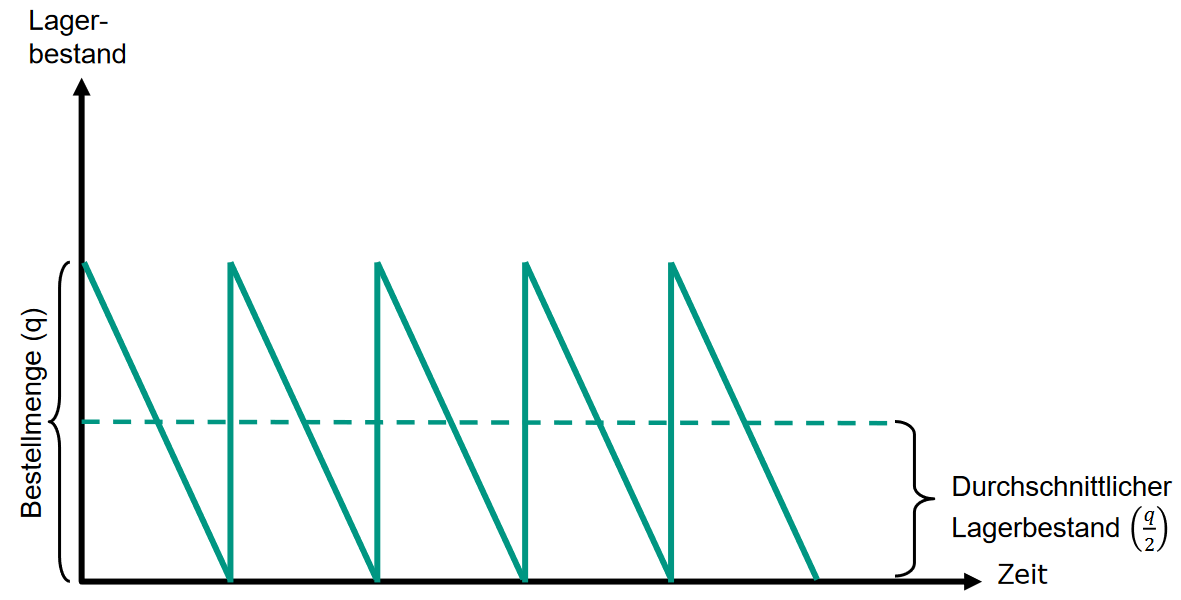
\includegraphics[width=0.7\textwidth]{images/lagerbestandsentwicklung.png}
\end{center}
\textbf{Ziel}: Ermittlung der optimalen Bestellmenge $q$

\textbf{Elemente}: 
\begin{itemize}
	\item Lagerung eines Gutes zum Stückpreis von $p$ mit Jahresbedarf $D$ Stück $\rightarrow$ \textbf{unmittelbare Beschaffungskosten} $K_u$
	\item Bestellfixe Kosten $K_f$ für jede Bestellung $\rightarrow$ \textbf{Bestellkosten} $K_q$
	\item Lagerkosten in Höhe des Zins- und Lagerkostensatzes $h$ $\rightarrow$ \textbf{Lagerkosten} $K_l$
	\item Zahl der Bestellvorgänge pro Jahr: $D/q$
	\item \textbf{Gesamtkosten}: $K=K_u+K_q+K_l$
	\begin{center}
		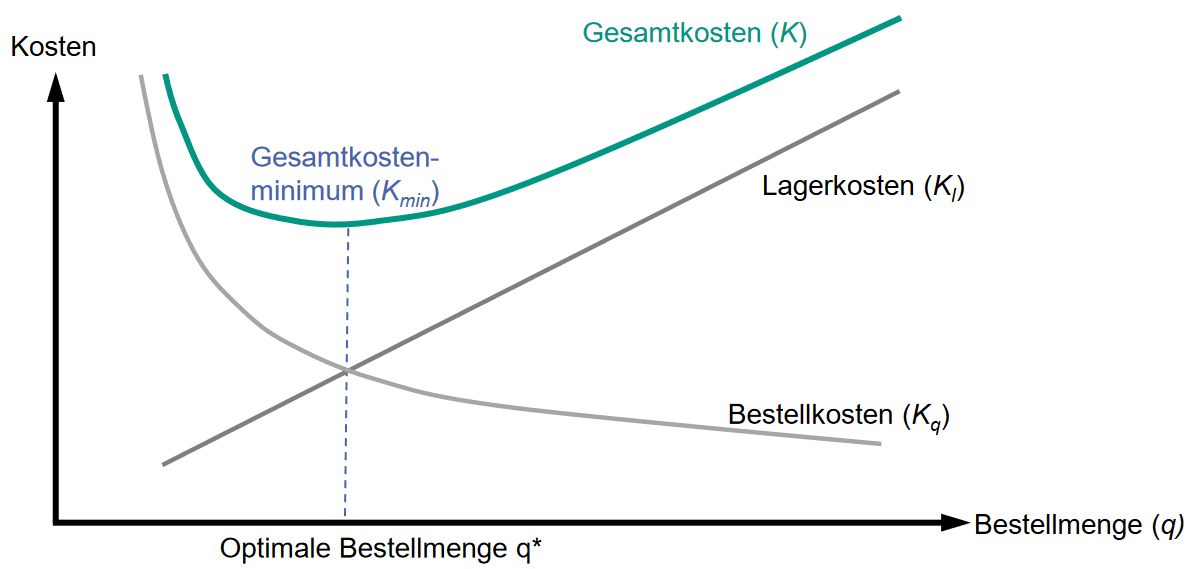
\includegraphics[width=0.7\textwidth]{images/haa.png}
	\end{center}
	\textbf{Es lässt sich herleiten}: $q^*=\sqrt{\frac{2DK_f}{ph}}$
	\item Beispielrechnungen: \textit{siehe Produktion Tut 2 oder VL 2, F50-52}
\end{itemize}

\textbf{Kritik}: Starke Annahmen des Modells führt zu Realitätsferne\\

\textbf{Unsicherheitsfaktoren für die Lagerhaltung:} 
\begin{itemize}
	\item Schwankungen der Nachfrage über die Perioden
	\item Schwankungen der Wiederbeschaffungszeit
	\item Schwankungen der Liefermenge
	\item Ungenauigkeiten der Bestandsführung
\end{itemize}
$\rightarrow$ Berücksichtigung stochastischer Periodenbedarfe durch einen
Sicherheitsbestand und in \textbf{Lagerhaltungspolitiken}

\subsection{Bestandsplanung}